\section{Asignación por centroide y validación}

\subsection{Procedimiento}
Para cada uno de los 170 municipios PDET se ejecutó un \texttt{updateMany}
con \texttt{\$geoWithin} sobre el campo \texttt{centroide} y el filtro
\texttt{cod\_mpio: null}, en \texttt{edificios\_google} y
\texttt{edificios\_microsoft}. El filtro evita reasignar edificios ya
asignados y se midió el tiempo por fuente. La ejecución quedó registrada
en \texttt{bitacora\_cargas}.

\subsection{Resultados de la asignación}
\begin{table}[H]
\centering\small
\caption{Asignación de edificios a municipios por centroide.}
\label{tab:asignacion}
\begin{tabular}{@{}lrrrrr@{}}
\toprule
\textbf{Fuente} & \textbf{Edificios} & \textbf{Asignados} & \textbf{Sin municipio} & \textbf{\% sin} & \textbf{Tiempo (s)} \\
\midrule
Google & 2\,694\,786 & 2\,694\,785 & 1 & 0,0\,\% & 269,9 \\
Microsoft & 1\,761\,048 & 1\,761\,048 & 0 & 0,0\,\% & 182,1 \\
\bottomrule
\end{tabular}
\end{table}


La asignación de Google (2.694.786 edificios) tardó 269,9\,s y la de
Microsoft (1.761.048 edificios), 182,1\,s. En Microsoft todos los edificios
quedaron asignados; en Google, 2.694.785 de 2.694.786.

\begin{figure}[h]
  \centering
  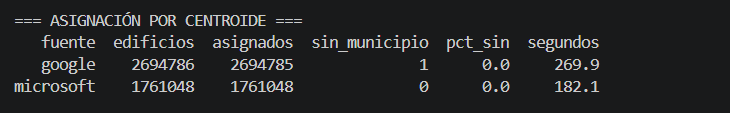
\includegraphics[width=\linewidth]{img/cap_asignacion.png}
  \caption{Salida de la asignación por centroide.}
\end{figure}

\subsection{Edificios sin municipio}
Un único edificio de Google (0,000037\,\%) quedó con \texttt{cod\_mpio: null}.
Su centroide (-72,97638; 9,15139) está a 0,011\,m del límite del municipio de
Convención (54206), es decir, prácticamente sobre la frontera. En un caso
así, la diferencia entre las aristas geodésicas que usa \texttt{\$geoWithin}
sobre la esfera y las aristas planas de la geometría puede decidir si el
punto queda dentro o fuera. En Microsoft no hubo ningún caso.

\subsection{Plan de ejecución: IXSCAN frente a COLLSCAN}
Se ejecutó \texttt{explain("executionStats")} sobre una consulta
\texttt{\$geoWithin} para el municipio de Caldono (19137), primero con el
índice \texttt{centroide\_2dsphere} y luego forzando
\texttt{hint(\{\$natural: 1\})}.

\begin{table}[H]
\centering\small
\caption{\texttt{explain("executionStats")} de \texttt{\$geoWithin} sobre \texttt{centroide}: con el índice y forzando \texttt{COLLSCAN}.}
\label{tab:explain-geowithin}
\begin{tabular}{@{}llrrrr@{}}
\toprule
\textbf{Fuente} & \textbf{Plan} & \textbf{Devueltos} & \textbf{Claves} & \textbf{Docs examinados} & \textbf{ms} \\
\midrule
Google & IXSCAN & 15\,303 & 25\,103 & 25\,071 & 730 \\
Google & COLLSCAN & 15\,303 & 0 & 2\,694\,786 & 7\,310 \\
Microsoft & IXSCAN & 12\,547 & 19\,460 & 19\,428 & 749 \\
Microsoft & COLLSCAN & 12\,547 & 0 & 1\,761\,048 & 4\,538 \\
\bottomrule
\end{tabular}
\end{table}


Con el índice, la consulta de Google examinó 25.071 documentos en 730\,ms;
sin él, recorrió los 2.694.786 documentos en 7.310\,ms, es decir, 107 veces
más documentos y 10 veces más tiempo. En Microsoft, 19.428 documentos en
749\,ms frente a 1.761.048 en 4.538\,ms (91 veces más documentos y 6 veces
más tiempo). Ambas variantes devolvieron los mismos resultados (15.303 y
12.547 edificios). El índice examina más documentos que los devueltos
porque primero filtra por celdas S2 y luego verifica la geometría exacta.

\begin{figure}[h]
  \centering
  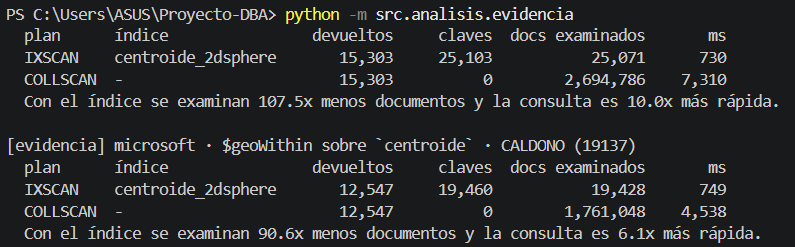
\includegraphics[width=\linewidth]{img/cap_explain_geowithin.png}
  \caption{\texttt{explain("executionStats")} con \texttt{IXSCAN} y con \texttt{COLLSCAN}.}
\end{figure}

\subsection{Validación independiente con GeoPandas}
Se validó una muestra de 10 municipios: dos del Chocó, tres grandes, tres
pequeños y dos sin edificios de Google (Murindó y Vigía del Fuerte). Los
centroides se cruzaron contra los límites con
\texttt{sjoin(predicate="within")} y se compararon los conteos con los de
MongoDB.

\begin{table}[H]
\centering\small
\caption{Validación: edificios por municipio en MongoDB frente a GeoPandas.}
\label{tab:validacion-asignacion}
\begin{tabular}{@{}lllrrr@{}}
\toprule
\textbf{Municipio} & \textbf{Categoría} & \textbf{Fuente} & \textbf{MongoDB} & \textbf{GeoPandas} & \textbf{Dif.} \\
\midrule
EL LITORAL DEL SAN JUAN & Chocó & Google & 309 & 309 & +0 \\
RIOSUCIO & Chocó & Google & 1\,000 & 1\,000 & +0 \\
SAN VICENTE DEL CAGUÁN & grande & Google & 21\,599 & 21\,599 & +0 \\
SOLANO & grande & Google & 6\,067 & 6\,067 & +0 \\
SAN JOSÉ DEL GUAVIARE & grande & Google & 32\,695 & 32\,695 & +0 \\
MANAURE BALCÓN DEL CESAR & pequeño & Google & 5\,951 & 5\,951 & +0 \\
COLOSO & pequeño & Google & 6\,278 & 6\,278 & +0 \\
CHALÁN & pequeño & Google & 3\,144 & 3\,144 & +0 \\
MURINDÓ & sin Google & Google & 0 & 0 & +0 \\
VIGÍA DEL FUERTE & sin Google & Google & 0 & 0 & +0 \\
EL LITORAL DEL SAN JUAN & Chocó & Microsoft & 2\,010 & 2\,010 & +0 \\
RIOSUCIO & Chocó & Microsoft & 6\,107 & 6\,107 & +0 \\
SAN VICENTE DEL CAGUÁN & grande & Microsoft & 23\,587 & 23\,587 & +0 \\
SOLANO & grande & Microsoft & 6\,171 & 6\,171 & +0 \\
SAN JOSÉ DEL GUAVIARE & grande & Microsoft & 21\,446 & 21\,446 & +0 \\
MANAURE BALCÓN DEL CESAR & pequeño & Microsoft & 3\,441 & 3\,441 & +0 \\
COLOSO & pequeño & Microsoft & 3\,999 & 3\,999 & +0 \\
CHALÁN & pequeño & Microsoft & 1\,902 & 1\,902 & +0 \\
MURINDÓ & sin Google & Microsoft & 1\,331 & 1\,331 & +0 \\
VIGÍA DEL FUERTE & sin Google & Microsoft & 1\,714 & 1\,714 & +0 \\
\bottomrule
\end{tabular}
\end{table}


En las 20 comparaciones (10 municipios por 2 fuentes) la diferencia fue 0,
sin edificios exclusivos de MongoDB ni de GeoPandas. Los dos municipios sin
Google dieron 0 en ambos métodos, y para Microsoft coincidieron en 1.331 y
1.714 edificios. Así, la asignación en MongoDB coincide con una
implementación independiente en el plano. La muestra no incluye el edificio
de Convención, por lo que el efecto de borde descrito arriba no aparece en
esta tabla.
